%%%%%%%%%%%%%%%%%%%%%%%%%%%%%%%%%%%%%%%%%%%%%%%%%%%%%%%%%%%%%%%%%%%%%%%%%%%%%%%%%%%%
% Document data
%%%%%%%%%%%%%%%%%%%%%%%%%%%%%%%%%%%%%%%%%%%%%%%%%%%%%%%%%%%%%%%%%%%%%%%%%%%%%%%%%%%%
\documentclass[12pt]{article} %report allows for chapters
%%%%%%%%%%%%%%%%%%%%%%%%%%%%%%%%%%%%%%%%%%%%%%%%%%%%%%%%%%%%%%%%%%%%%%%%%%%%%%%%%%%%
\usepackage{preamble}

\begin{document}

\begin{center}
   \textsc{\large MATH 271, Homework 1, \emph{Solutions}}\\
\end{center}
\vspace{.5cm}

\begin{problem}
    Look up how to do \emph{integration by parts}. Use this technique to compute the integral
    \[
        \int t e^{3t}dt.
    \]
\end{problem}

\begin{solution}
    Integration by parts is a combination of the derivative product rule and the fundamental theorem of calculus.  Given functions $u(x)$ and $v(x)$ we can write
    \[
    (uv)'=u'v+uv'.
    \]
    Then if we integrate both sides, we have
    \[
    \int_a^b (uv)'dx = \int_a^b u'vdx + \int_a^b uv'dx.
    \]
    Fundamental theorem of calculus gives us that
    \[
    \int_a^b (uv)'dx = u(b)v(b)-u(a)v(a)
    \]
    and thus
    \[
    \int_a^b u'vdx = u(b)v(b)-u(a)v(a)-\int_a^b uv'dx.
    \]
    Or, without bounds on the integral, we can write
    \[
    \int u'vdx = uv - \int uv'dx.
    \]
    I like to think of integration by parts as shifting the derivative from one function to another with a penalty term.  Above, we swap a derivative on $u$ to a derivative on $v$ but have to correct with the function $uv$.  This can all be derived in higher dimensions using Stokes' theorem. It's an excellent tool in the study of differential equations.
    
    Now, the technique to doing integration by parts is to identify a function that when we take its derivative it gets simpler.  So, in our integral
    \[
    \int te^{3t}dt
    \]
    we have that $t$ is a function that gets simpler when we take its derivative. That is, $\frac{d}{dt}t=1$. So, I'll let $u'=e^{3t}$ and $v=t$.  Then we have $u=\frac{1}{3}e^{3t}$ and $v'=1$. Let's replace these into our formula
    \begin{align*}
        \int u'vdt &= uv - \int uv'dt\\
        \int e^{3t}tdt &= \frac{t}{3}e^{3t} - \int \frac{1}{3}e^{3t}\cdot 1 dt\\
        &= \frac{t}{3} e^{3t} - \frac{1}{9}e^{3t}+c\\
        &= \left( \frac{t}{3}-\frac{1}{9}\right)e^{3t}+c.
    \end{align*}
\end{solution}
\newpage

\begin{problem}
Convert the following numbers in Cartesian coordinates to polar coordinates and compute all pairwise products.
\begin{enumerate}[(a)]
    \item $z_1=\frac{1}{2}-\frac{1}{2}i$;
    \item $z_2=-1+3i$;
    \item $z_3=-2-3i$.
\end{enumerate}
\end{problem}

\begin{solution}~
\begin{enumerate}[(a)]
    \item We have that
    \[
    r=\sqrt{z_1z_1^*}=\sqrt{\frac{1}{4}+\frac{1}{4}}=\frac{1}{\sqrt{2}}
    \]
    and since $a>0$, 
    \[
    \theta = \arctan\left( \frac{1/2}{-1/2}\right)=-\frac{\pi}{4}.
    \]
    So
    \[
    z_1 = \frac{1}{\sqrt{2}} e^{-i\frac{\pi}{4}}.
    \]
    \item We have $a<0$ so
    \[
    r=\sqrt{10} \qquad \textrm{and} \qquad \theta = \arctan\left( \frac{3}{-1}\right)+\pi
    \]
    giving us that
    \[
    z_2 \approx \sqrt{10}e^{1.893i}.
    \]
    \item Again, $a<0$ so we have,
    \[
    r=\sqrt{13} \qquad \textrm{and} \qquad \theta = \arctan \left(\frac{-3}{-2}\right)+\pi.
    \]
    Hence,
    \[
    z_3 \approx \sqrt{13}e^{4.124i}.
    \]
\end{enumerate}
Now we can compute all pairwise products.
\begin{align*}
    z_1 z_2 &= 1+2i\approx 2.236e^{1.107i}\\
    z_1 z_3 &= \frac{1}{2}-\frac{5}{2}i\approx 2.550e^{-1.373i}\\
    z_2 z_3 &= 11-3i\approx 11.402e^{-0.266i}.
\end{align*}

\end{solution}

\newpage

\begin{problem}
Find the square roots of $-i$ using a geometrical argument.
\end{problem}

\begin{solution}
Thinking of $-i=e^{i\frac{3\pi}{2}}$ we can find the square root by finding a number that has a half this rotation in a clockwise way, or a counter clockwise way.  So, we have
\[
\sqrt{-i}=e^{i\frac{3\pi}{4}}
\]
and
\[
\sqrt{-i}=e^{-i\frac{\pi}{4}}.
\]
Here's a picture to illustrate this.
 \begin{center}
            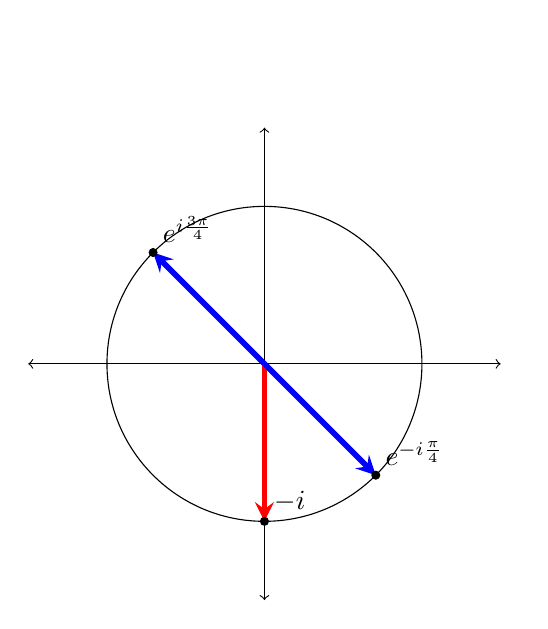
\begin{tikzpicture}
            \draw[<->] (-3,0)--(3,0) node[right]{$\RE$};
            \draw[<->] (0,-3)--(0,3) node[above]{$\IM$};
            \tdplotdrawarc[->,line width = 1pt, black]{(0,0)}{1}{0}{270}{}{};
            \node[anchor=east] at (-.75,1){};
            \tdplotdrawarc[->,line width = 1pt, black]{(0,0)}{1.3}{0}{135}{}{};
            \node[anchor=west] at (1.4,.5){};
            \tdplotdrawarc[->,line width = 1pt, black]{(0,0)}{.5}{0}{-45}{}{};
            \node[anchor=north east] at (-1,-1){};
            \draw[line width=2pt,red,-stealth](0,0)--(0,-2) node[anchor=south east] at (0,4){};
            \draw[line width=2pt,blue,-stealth](0,0)--(-1.414,1.414) node[anchor=south east] at (2.828,2.828){};
            \draw[line width=2pt,blue,-stealth](0,0)--(1.414,-1.414) node[anchor=south west] at (1,1){};
            \foreach \Point/\PointLabel in {(0,-2)/{-i}, (-1.414,1.414)/{e^{i\frac{3\pi}{4}}}, (1.414,-1.414)/{e^{-i\frac{\pi}{4}}}}
            \draw[fill=black] \Point circle (0.05) node[anchor=south west] {$\PointLabel$};
            \draw (0,0) circle (2);
            \end{tikzpicture}
        \end{center}
\end{solution}

\newpage

\begin{problem}
Draw the unit circle in the complex plane. Plot the complex numbers $z_1$ and $z_2$ given above and find their inverses and conjugates. Explain what taking the inverse and conjugate does geometrically.
\end{problem}

\begin{solution}
From the previous problem we had
\begin{align*}
z_1 &= \frac{1}{2}-\frac{1}{2}i = \frac{1}{\sqrt{2}}e^{-i\frac{\pi}{4}}\\
z_2 &= -1 + 3i \approx \sqrt{10}e^{-1.893i}.
\end{align*}
Recall that the inverse for a complex number $z=a+bi=re^{i\theta}$ is given by
\[
z^{-1}=\frac{z^*}{\|z\|^2}=\frac{a}{a^2+b^2}-\frac{bi}{a^2+b^2}
\]
or in polar coordinates by
\[
z^{-1}=\frac{1}{r}e^{-i\theta}.
\]
So we have the inverses
\begin{align*}
    z_1^{-1} &= 1+i = \sqrt{2}e^{i\frac{\pi}{4}}\\
    z_2^{-1} &= \frac{-1}{10}-\frac{3i}{10} \approx \frac{1}{\sqrt{10}} e^{1.893i}
\end{align*}
and the conjugates
\begin{align*}
    z_1^* &= \frac{1}{2}+\frac{1}{2}i = \frac{1}{\sqrt{2}}e^{i\frac{\pi}{4}}\\
    z_2^* &= \frac{-1}{10}+\frac{3i}{10} \approx \frac{1}{\sqrt{10}} e^{-1.893i}
\end{align*}
    \begin{center}
            \begin{tikzpicture}[scale=.75]
            \draw[<->] (-10,0)--(10,0) node[right]{$\RE$};
            \draw[<->] (0,-10)--(0,10) node[above]{$\IM$};
            \foreach \Point/\PointLabel in {(1.5,-1.5)/{z_1}, (-3,9)/{z_2}, (3,3)/{{z_1}^{-1}}, (-.3,-.9)/{z_2^{-1}},(1.5,1.5)/{z_1^*}, (-3,-9)/{z_2^*} }
            \draw[fill=black] \Point circle (0.05) node[anchor=east] {$\PointLabel$};
            \draw (0,0) circle (3);
            \end{tikzpicture}
        \end{center}
    Geometrically what the inverse does is reverses the angle (or argument) $\theta$ of the complex number to $-\theta$ and scales the length $r$ by $1/r$. 
\end{solution}
\newpage

\begin{problem}
    What is an (ordinary) differential equation? Explain what it means to be a general and particular solution to a differential equation.
\end{problem}
\begin{solution}
    An Ordinary Differential Equation (ODE) is an equation involving an unknown function $x(t)$ that depends on one independent variable $t$.  We tend to think of the dependent variable $x$ as representing position and we think of the independent variable $t$ as representing time.

    A general solution is a function $x(t)$ that solves an ODE. These general solutions will have undetermined constants.  Specifically, there will be an unknown constant for the order of the problem (e.g., a second order problem will have two unknown constants). When given initial conditions for an ODE, we call this an Initial Value Problem (IVP).  A particular solution is a solution to an IVP. That is, it not only solves the ODE, but satisfies the given initial conditions as well.  A particular solution is a single member of the set of general solutions.  

    The analogy is as follows: If a ball falls due to gravity, then I can determine a general solution that describes this.   If I then also provide the initial position and velocity of the ball, then I would know the exact trajectory of the ball.  This exact trajectory is a particular solution unique to those initial conditions.
\end{solution}


\newpage

\begin{problem}
    Look up a differential equation in chemistry that interests you.  Write it down, and explain what it attempts to model. Why does it interest you?
\end{problem}

\begin{solution}
    One that interests me is the \emph{Schr\"odinger equation}. It is useful in describing the motion of subatomic particles and gives rise to the structure of the hydrogen atom.  One can then expand a bit to study the helium atom and generalize this further to understand the whole of the periodic table.  The equation is, to me, a bit like a square root of a wave equation. The \emph{wave equation} is
    \[
    \nabla^2 f(\mathbf{r},t) = \frac{1}{c^2}\frac{\partial^2}{\partial t^2}f(\mathbf{r},t),
    \]
    which describes, for example, the vibration of a guitar string or ripples on the surface of a pool. The Schr\"odinger equation is 
    \[
    \left( \frac{-\hbar^2}{2m}\nabla^2 + V(\mathbf{r},t)\right) \Psi(\mathbf{r},t) = i\hbar \frac{\partial}{\partial t}\Psi (\mathbf{r},t).
    \]
    This equation is essentially the quantum version of Newton's law $F=ma$. The equation is very successful at modelling interactions of very small particles such as protons and electrons.  The function $V$ is an external potential which could come from, say, an electric field. When $V=0$, then we have something very similar to a wave equation. The function we wish to solve for is $\Psi$. However, $\Psi$ itself is not \emph{really} physical.  But, it gives rise to statistics which we can measure.  For example, if we have a solution $\Psi$ to the equation that describes the position of a particle, then
    \[
    \int_\Omega \Psi^*(\mathbf{r}',t) \Psi(\mathbf{r}',t) d\mathbf{r}'
    \]
    gives the probability of a particle being in the region $\Omega$ at time $t$.

    This equation interests me because it describes the world in the best detail that we know of.  Our beliefs in classical mechanics is simply not correct -- quantum mechanics shows us that our classical intuition has to be thrown out in the case of small particles and their interactions.  It's amazing to get to learn what happens on small scales and use this to understand, for example, the periodic table.
\end{solution}

\newpage

\begin{problem}
Objects near Earth fall due to gravity.  The acceleration of an object due to gravity is then
\[
y''=g,
\]
where $x$ represents the distance above the ground and $g\approx -9.8\frac{m}{s^2}$ is constant.  
\begin{enumerate}[(a)]
    \item Find the general solution to the equation.
    \item Given the initial data $y(0)=0$ and $y'(0)=1$, find the particular solution.
    \item At what time $t>0$ does the object first contact the ground?
    \item Plot your solution over the range of time that makes physical sense.
\end{enumerate}

\end{problem}
\begin{solution}~
\begin{enumerate}[(a)]
    \item This equation can be solved by integrating twice.  However, I like to make a substitution of $f=y'$ so that we can write
    \[
    f'=g.
    \]
    Now, this is a first order separable equation which we can solve by
    \begin{align*}
        \frac{df}{dt}&=g\\
        \int df&= \int gdt\\
        f&= gt+C_1.
    \end{align*}
    Now, since $y=x'$ we can look at
    \[
    y'=gt+C_1
    \]
    which is also separable.  We integrate and find
    \begin{align*}
        \frac{dy}{dt}&=gt+C_1\\
        \int dy &= \int gt+C_1 dt\\
        y(t)&= \frac{1}{2}gt^2+C_1t+C_2
    \end{align*}
    is our general solution.
    \item Now, we use our initial data along with our general solution
    \begin{align*}
        0=y(0)&=\frac{1}{2}g(0)^2+C_1(0)+C_2\\
        &=C_2.
    \end{align*}
    So $C_2=0$. Next, use the information about the first derivative $x'(0)=1$ and we have
    \begin{align*}
        1=y'(0)&=g(0)+C_1\\
        =C_1.
    \end{align*}
    Thus $C_1=1$. Now, our particular solution is
    \[
    \boxed{y(t)=\frac{1}{2}gt^2+t.}
    \]
    \item Now, the points at which the object is on the ground are the values of $t$ where $y(t)=0$ since $y$ represents the height above the ground.  So we have to solve
    \[
    0=y(t)=\frac{1}{2}gt^2+t=t\left(\frac{1}{2}gt+1\right).
    \]
    This has roots $t=0$ and $t=-\frac{2}{g}$.  So the time $t>0$ the ball hits the ground is $t=-\frac{2}{g} \approx 0.204$.
    \item Here's a plot of the solution from time $t=0$ until it hits the ground (see (d)).
    \begin{figure}[H]
        \centering
        \includegraphics[width=\textwidth]{projectile.png}
    \end{figure}
\end{enumerate}
\end{solution}

\end{document}